\subsection{Modellagnostische Methoden - global}
\subsubsection{Partial Dependence Plot}
\label{subsubsec_PDP}
Ein Partial Dependence Plot kann zur Visualisierung eingesetzt werden, nachdem ein Modell trainiert wurde \cite{Gianfagna.2021}. Sie verfolgt das Ziel aufzudecken, inwiefern Merkmale die Black-Box-Modell-Ausgaben beeinflussen. Diese Art der Darstellung misst, wie sich ein Merkmal auswirkt, wenn man den Wert diesen immer etwas abändert, aber die Werte der anderen Merkmale nicht modifiziert. \cite{kamath2021explainable}.
Vereinfacht gesagt würde man bei zwei Variablen, die jeweils z.B. einen möglichen Wert von 1-5 annehmen können, für das erste Merkmal das Modell mit dem Wert 0 aufrufen, während man das zweite Merkmal nicht verändert. Im nächsten Schritt würde man den Wert des ersten Merkmals auf 1 setzen usw. Ist dies für alle möglichen Werte des ersten Merkmals geschehen, wird der Mittelwert der Vorhersagen berechnet. Dies wird daraufhin für das zweite Merkmal wiederholt. 
Formal ist die PD definiert mit $d$ als Anzahl der Merkmalen (\cite{kamath2021explainable} nach \cite{friedman2001greedy}): 
\begin{equation}
    PD(x_{1}) = \mathds{E}_{x_{2}}[f(x_{1},x_{2})] = \int p(x_{2}) f(x_{1},x_{2})d_{x_{2}}
\end{equation}
Abbildung \ref{Fig:PDP_Beispiel} zeigt ein Beispiel für einen PDP. 
\begin{figure}[h]
    \centering
    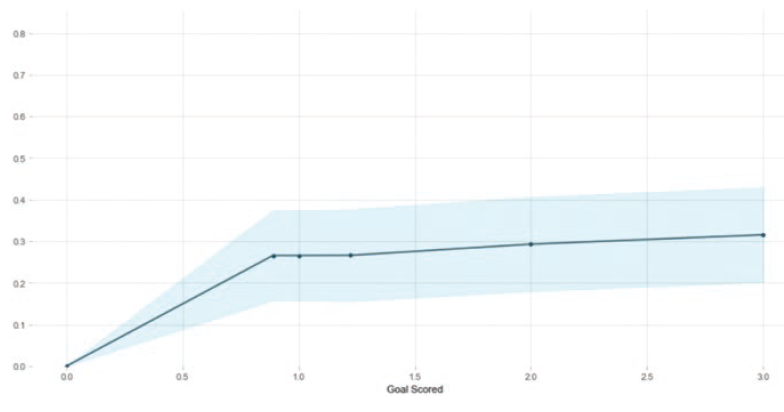
\includegraphics[scale=0.45]{pic/MA-Bilder/Literaturrecherche/PDP-Beispiel.PNG}
    \caption{Beispiel für einen PDP, entnommen aus: \cite{Gianfagna.2021}}
    \label{Fig:PDP_Beispiel}
\end{figure}

%Für die Anwendung eines PDP existiert ein Modul von Scikit-Learn \footnote{https://scikit-learn.org/stable/modules/partial_dependence.html}
%Hiermit schaut man, welche Effekte Features auf den Output haben \cite{kamath2021explainable}, dies ist eine glibale Methode und zeigt Beziehungen zwischen den merkmalen in den Input und den Vorhersagen auf. PD-Diagramme visualisieren die partielle Abhängigkeitsfunktion, die die Wirkung eines Merkmals durch Abgrenzung über andere Merkmale misst. Bei einem Modell mit zwei Merkmalen, f (x1, x2), wird die partielle Abhängigkeitsfunktion des Merkmals x1 beispielsweise durch Mittelung über die Randverteilung des Merkmals x2

Ein Vorteil der PDP-Methode ist es weniger zu zeigen, welches Merkmal den größten Einfluss auf eine Vorhersage hat (wie z.B. die Methode der Permutation Importance \todo{dazu muss ich noch ein Kapitel schreiben}), sondern bestimmte Schwellenwerte aufzudecken. So können PDP dabei helfen, zu definieren, wie ein Wert eines Merkmals besetzt sein sollte, um ein bestimmtes Ergebnis zu bekommen \cite{Gianfagna.2021}. 
%Youtube-Video(https://www.youtube.com/watch?v=uQQa3wQgG_s):
%Man hat die Datensätze mit den Features, Beispiel: alle Features haben Werte von 0-5 oder so, dann setzt man von EINEM Feature alle diese Werte von dem Feature auf 0 --> dann berechnet man (mit den anderen Features zusammen),was jeweils raus kommt (Rest der Daten bleibt gleich) --> dann hat man ganz viele Vorhersagen und nimmt dann die Average von den ganzen --> dann wei0 man, wie das die Vorhersage beeinflusst, wenn der Wert des Features 0 war --> dann setzt man das auf 1 und berechnet die Average und so weiter
%dann plottet man das und sieht halt --> Average Vorhersage, wenn Feature 0,1,2,3,4,5 war
%Das macht man halt mit allen Features
Ein Nachteil dieser Methode beruht auf der Annahme, dass die Merkmale unabhängig voneinander sind. So wird, wie oben erklärt, der Wert des ersten Features nach Belieben geändert, während der Wert des zweiten Features gleich bleibt. Jedoch führt dies zu Kombinationen, welche in der Realität nicht vorkommen können \cite{molnar2022}.
%Youtube-Video:
%Nachteil der Average-Funktion: starke Vereinfachung, wäre cool zu sehen, ob die verschiednene Predicted Values sehr stark aneinander liegen oder eben nciht (man könnte Verteilung darstellen, anstatt nur die Punkte)
%Hier Beispiel einfügen: 

Eine weitere ähnliche Methode ist der \emph{Accumulated Local Effects (ALE) Plot} nach \textcite{apley2020visualizing}, welches das Problem der Abhängigkeit löst.
%TODO das vlt. noch machen, gutes, aber langes Video hier: https://www.youtube.com/watch?v=06knUxoig9Y

\subsubsection{Individual Conditional Expectation (ICE)}
\begin{figure}[h]
    \centering
    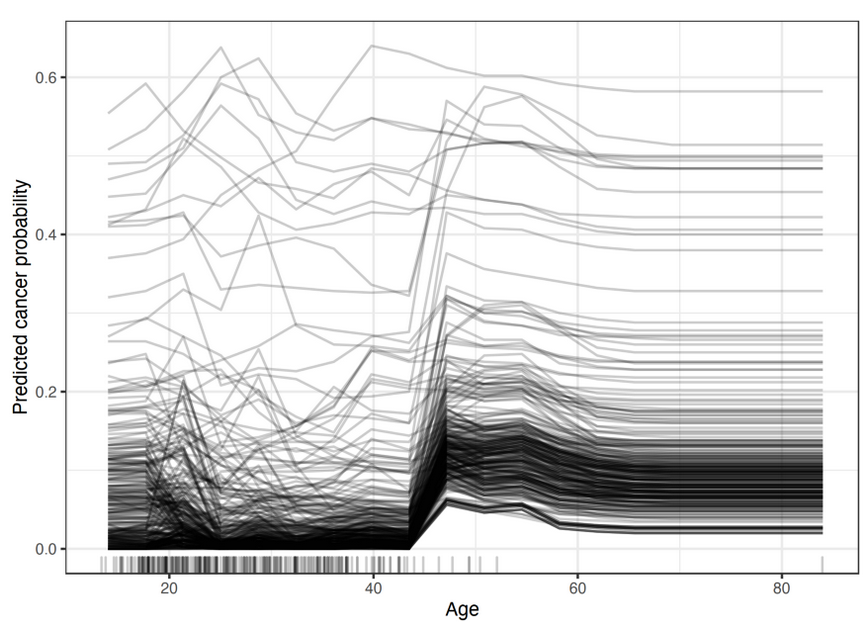
\includegraphics[scale=0.35]{pic/MA-Bilder/Literaturrecherche/ICE_Beispiel.PNG}
    \caption{Beispiel für ICE, entnommen aus: \cite{ICE-beispiel}}
    \label{Fig:Beispiel_ICE}
\end{figure}
Die Funktionsweise der ICE-Methode ist die selbe der PDP (vgl. Unterkapitel \ref{subsubsec_PDP}), wir hier jedoch lokal anstatt global angewendet, indem die Werte für jede Instanz berechnet werden \cite{molnar2022}. Somit lassen sich der Einfluss von Änderungen einzelner Features bestimmen \cite{hanif2021survey}. Nach \textcite{molnar2022} ist ein PDP ein Mittelwert der ICE. ICE kann jedoch eine gute Alternative bieten, tiefere Einblicke in die Feature-Interaktionen zu erhalten \cite{molnar2022}. In Abbildung \ref{Fig:Beispiel_ICE} ist ein Beispiel für eine ICE zu sehen: 

\subsubsection{Global Surrogate}
Um jedes beliebige Black-Box-Modell zu erklären, kann ein interpretierbares Modell eingesetzt werden, welches sich dem ursprünglichen Modell annähert. Diese Methode heißt Global Surroagte (globaler Stellvertreter) \cite{molnar2022}. In Kapitel \ref{subsubse_LIME} ist dieses Konzept lokal beschrieben. Ziel dieser Methode ist eine ungefähre Abschätzung des ursprünglichen Modells, während Interpretierbarkeit gewährleistet wird. Entscheidend bei dieser Methode ist die Wahl des Modells, denn dieses muss interpretierbar sein. Eine Auswahl von transparenten Modellen ist in Kapitel \ref{subsubsec_transparenteModelle} zu finden, so sind bspw. lineare Modelle oder Entscheidungsbäume geeignet \cite{molnar2022}.

Die Implementation eines solchen globalen Stellvertretermodells ist relativ simpel, so wird kein Zugriff und auch kein Wissen über die Modellstruktur benötigt. Entwickler, welche einen globalen Stellvertreter entwickeln wollen, müssen sich zunächst für einen Datensatz entscheiden und für diesen die Vorhersagen abrufen. Im nächsten Schritt wird sich für ein interpretierbares Modell entschieden, welches dann auf die ursprünglichen Daten und Vorhersagen trainiert wird. Daraufhin findet eine Evaluation statt \cite{molnar2022}.

Eine Möglichkeit, zu überprüfen, wie exakt der Stellvertreter das Black-Box-Modell annähert, ist das $R^{2}$-Maß, welches wie folgt definiert ist:
%SSE ist Summe von Squares Error und SST ist Summe of Squares Gesamt (1-\frac{SSE}{SST}=)
\begin{equation}
    1-\frac{\sum_{i=1}^n(\hat{y}_{*}^{(i)}-\hat{y}^{(i)})^{2}}{\sum_{i=1}^n(\hat{y}^{(i)}-\bar{\hat{y}})^{2}}
\end{equation}

Die Vorhersage des interpretierbaren Modells ist für die i-te Instanz $\hat{y}_{*}^{(i)}$, während die Vorhersage des Urpsrungmodells mit $\hat{y}^{(i)}$ notiert ist. $\bar{\hat{y}}$ gibt den Mittelwert der Vorhersagen des Black-Box-Modells an. Wenn sich das Ergebnis in der Nähe von 1 befindet, ist dies so zu verstehen, dass der Stellvertreter sich dem Modell gut annähert. Nähert sich der Stellvertreter sehr gut an, kann sogar in Betracht gezogen werden, dieses anstatt des ursprünglichen Modells zu verwenden. Liegt der Wert nahe bei 0, bedeutet dies analog, dass sich das Stellvertretermodell nicht eignet \cite{molnar2022}. %R sagt nix über die Performance des Black-Box-Modells aus, sondern nur wie gut der Stellvertreter das immitiert.

Ein Vorteil dieser Methode ist dessen einfache Anwendung. Daneben kann flexibel jedes mögliche Modell als Stellvertreter gewählt werden. So kann sowohl auf die Kenntnisse der Entwickler als auch auf die der Nutzer eingegangen werden. Wenn alle Stakeholder sich z.B. gut mit Entscheidungsbäumen auskennen, kann dieses Modell als Stellvertreter gewählt werden. Daneben existieren natürlich auch Nachteile dieser Methode. Jedes interpretierbare Modell bringt selbst seine eigenen Schwächen mit und es werden Annahmen über das Black-Box-Modell getroffen, welche eventuell nicht der Wahrheit entsprechen. Dazu kann es eine schwierige Entscheidung sein, welcher $R^{2}$-Wert als ausreichend betrachtet wird.

\subsubsection{Protoypen und Kritiken}
XAI-Modelle können auch mit konkreten Dateninstanzen erklärt werden. Als Protoypen werden solche Instanzen bezeichnet, die einen Datensatz repräsentieren, während Kritiker solche Datenpunkte sind, welche schlecht die gesamten Datensätzen wiedergeben. %(https://christophm.github.io/interpretable-ml-book/proto.html#proto)
Mit diesen Konzepten lassen sich sowohl Datensätze als auch ML-Modelle erklären, was in Abbildung \ref{Fig:Prototyp_Kritiekr} dargestellt ist für Instanzen, welche die Merkmale $x1$ und $x2$ in unterschiedlicher Ausprägung besitzen \cite{molnar2022}.
\begin{figure}
    \centering
    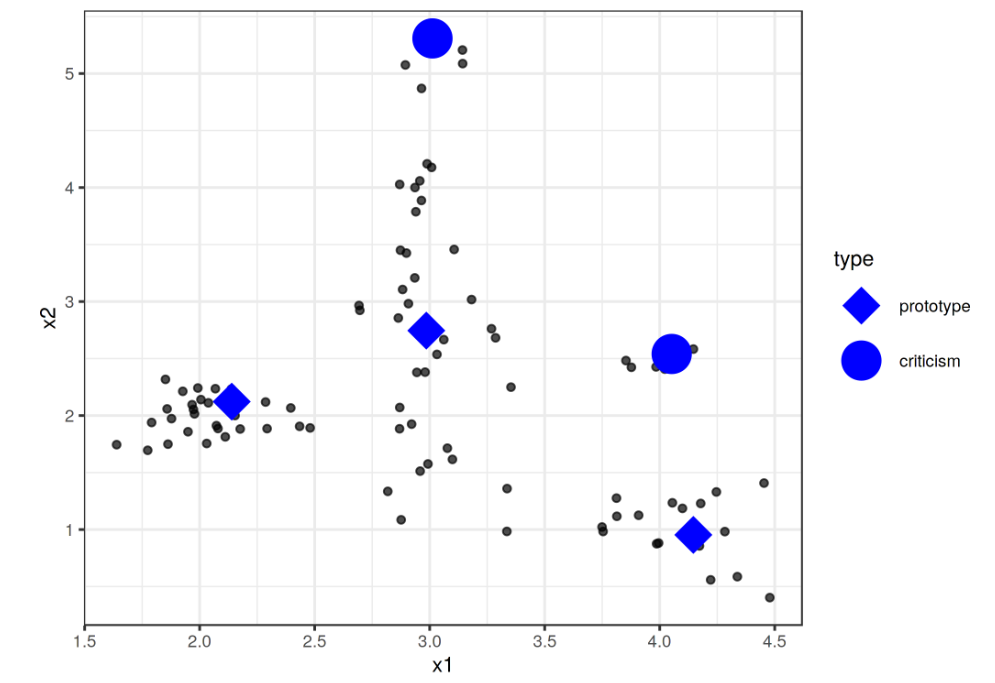
\includegraphics[scale=0.45]{pic/MA-Bilder/Literaturrecherche/Prototyp_Kritiker-Beispiel.PNG}
    \caption{Protoypen und Kritker, entnommen aus: \cite{molnar2022}}
    \label{Fig:Prototyp_Kritiekr}
\end{figure}
Zum Finden dieser Datenpunkte existieren verschiedene Methode. Die einfachste Methode stammt von \textcite{rdusseeun1987clustering}, lässt sich jedoch nur für Protoypen anwenden. Diese Methode heißt \emph{k-medoids} und funktioniert ähnlich zu der in Kapitel \ref{subsubsec:k-means-Clustering} beschriebenen Methode k-means Clustering. Eine weitere Methode, die sowohl das Identifzieren von Protoypen als auch Kritiker ermöglicht, heißt \emph{MMD-critic} und wurde von \textcite{kim2016examples} vorgestellt. % Das kann man auch direkt benutzen: %https://github.com/BeenKim/MMD-critic und hier: Recently an extension of MMD-critic was developed: Protodash. The authors claim advantages over MMD-critic in their publication. A Protodash implementation is available in the IBM AIX360 tool.
\todo[inline]{Hier kommt noch eine Beschreibung der MMD-Critic-Methode}